\documentclass[a4paper,12pt]{article}

\usepackage[russian]{babel}
\usepackage{cmap}
\usepackage[utf8]{inputenc}
\usepackage[usenames]{color}
\usepackage{tabularray}
\usepackage{xcolor}
\usepackage{graphicx} 
\usepackage{subfigure}
\usepackage{subcaption}

\usepackage[unicode]{hyperref} % цвета гиперссылок
\hypersetup{
	colorlinks,
	citecolor=black,
	filecolor=black,
	linkcolor=blue,
	urlcolor=black
}

\usepackage{geometry} % задаёт поля 
%\geometry{left=3cm}
%\geometry{right= 1.5cm}
%\geometry{top=2cm}
%\geometry{bottom=2cm} 

\usepackage{enumitem} % настраивает работу со списками:
\def\labelitemi{—} % ... задаёт длинное тире как стандартный маркер ненумерованного списка
\setlist{nolistsep} %  ... убирает дополнительный отступы между элементами списка


% удаляет названия и продолжение следует и т. для таблиц, будет только таблица без всего
\DefTblrTemplate{contfoot-text}{default}{}
\DefTblrTemplate{conthead-text}{default}{}
\DefTblrTemplate{caption}{default}{}
\DefTblrTemplate{conthead}{default}{}
\DefTblrTemplate{capcont}{default}{}


\title{Об одной метрике эффективности агломеративной кластеризации }
\author{В. Г. Мосин}
\date{}

%   \input{preamble.tex}
\begin{document}
	\maketitle
	\abstract{\noindent  Излагается метод оценки эффективности агломеративной кластеризации, основанный на вычислении средней дистанции между центроидами кластеров на обучающей и тестовой выборке. Приводится алгоритм метода. Рассматривается пример подбора оптимальной кластеризации данных о потреблении контента.  }
	
\tableofcontents
	
\section{Введение}
Кластеризация данных — это метод машинного обучения, осуществляющий группировку данных на основе их схожести (см. [5]). В процессе кластеризации данные разделяются на группы, которые называются кластерами, таким образом, что объекты внутри одного кластера более похожи друг на друга, чем на объекты из других кластеров. Кластеризация позволяет выявить скрытые шаблоны, структуры и взаимосвязи в данных, которые могут быть незаметны при первом взгляде. Путем группировки по схожести можно выделить группы схожих объектов и выделить ключевые особенности каждой группы (см. [5], [6]).

Определение числа кластеров является важным элементом анализа данных. 
Во-первых, число кластеров напрямую влияет на качество и интерпретируемость кластеризации. Неправильное определение числа кластеров может привести к объединению сильно различающихся групп в один кластер или к разделению однородной группы на несколько кластеров. Правильно определенное число кластеров помогает обнаружить скрытые шаблоны, взаимосвязи и сходства в данных. 

Далее, разбиение данных на недостаточное число кластеров может привести к упрощению кластерной структуры, не раскрывающей всю информацию в данных. Хотя, с другой стороны, слишком большое число кластеров может привести к излишней сложности и непонятности кластеризации. Определение оптимального числа кластеров помогает найти баланс между этими двумя крайностями. 

И, наконец, существенным является вопрос принятия решений. Определение правильного числа кластеров помогает принимать правильные решения на основе кластерного анализа, такие как создание сегментов покупателей, выявление характерных поведенческих паттернов или предсказание рисков и мошеннических действий.

В целом, определение числа кластеров является важным этапом в анализе данных, который помогает найти баланс между сложностью и информативностью кластеризации, а также позволяет принимать правильные решения на основе результатов анализа.


\subsection{Теоретическая часть}

Как правило, кластеризация осуществляется на основании мнения исследователя или представителя экспертной группы из конкретной предметной области, к которой относятся анализируемые данные (см. [5], [6]). В таком случае, ответственность за качество кластеризации ложится на исследователя или эксперта, и вопрос о машинно-ориентированном подходе к оценке качества кластеризации не возникает вообще.

Однако, в ряде случаев такой подход невозможен или нецелесообразен. Известные методы кластеризации, такие как KMeans или агломеративная кластеризация, формируют кластеры самостоятельно, отталкиваясь от геометрической близости (или отдаленности) объектов, но они требуют указания априорных значений своих параметров, в первую очередь, числа кластеров, которое опять-таки выбирается субъективно.

Таким образом, есть насущная необходимость в некоторой метрике, которая позволяла бы сравнивать качество кластеризации при изменении количества используемых кластеров, и в настоящей работе мы предлагаем такую метрику.

\subsection{Постановки задачи}

\subsubsection{Предмет исследования}

Предметом исследования служит метод, определяющий оптимальное число кластеров для агломеративной кластеризации. 

\subsubsection{Методика исследования} 

Мы разбиваем облако данных на две выборки, которые называем обучающей и тестовой, и производим их кластеризации. Если число кластеров подобрано хорошо, то кластеризации на этих двух выборках будут «похожими» друг на друга, и в качестве критерия их сходства мы предлагаем следующую идею.

Несмотря на то, что агломеративная кластеризации не апеллирует к понятию центроида кластера, после кластеризации все равно возникает несколько кластеров, каждый их которых обладает своим центроидом. Если центроиды на обучающей выборке и тестовой выборке расположены близко друг к другу, то кластеризация качественная, если они менее близки, то она менее качественна и так далее. Это соображение позволяет упорядочить кластеризации с различным количеством кластеров по метрике, в качестве которой мы принимает среднюю дистанцию между центроидами на обучающей и тестовой выборке.

\subsubsection{Цель исследования} 

Наша цель — реализовать метрику средних дистанций в виде алгоритма и провести апробацию метода.

\subsection{Библиотеки}
Для выполнения вычислений и анализа данных мы пользуемся средой \texttt{Jupyter Notebook}, которая предоставляет удобные средства для работы с языком программирования Python и его главными библиотеками: \texttt{NumPy}, \texttt{Pandas}, \texttt{sklearn} и \texttt{matplotlib}. Благодаря этим инструментам, мы можем эффективно работать с данными, выполнять исследования и визуализировать результаты (см. [1], [2]). 

Библиотека \texttt{numpy} является одной из ключевых библиотек для научных вычислений и обработки массивов данных в языке программирования \texttt{Python}. Библиотека \texttt{pandas}~--- одна из наиболее популярных и мощных библиотек для работы с данными в языке программирования \texttt{Python} (см. [1]). 

Библиотека \texttt{scikit-learn}, широко известная как \texttt{sklearn}, предоставляет обширный набор инструментов и функций для решения различных задач в языке программирования Python, таких как задачи классификации, регрессии, кластеризации и др. Мы используем эту библиотеку для решения регрессионных задач.

\section{Описание данных}
Для применения нашего алгоритма мы в качестве примера используем данные о потреблении контента пользователями одного из ведущих хостингом. Данные представляют собой записи о 500 датах, начиная с 2021-08-20 и заканчивая 2023-01-01. В каждую из этих дат были зафиксированы показатели потребления контента, такие, как 'Просмотры', 'Время просмотра (часы)', 'Поделились' и т. д. всего 18 признаков. Подробная структура данных описана ниже.
\section{Алгоритм}
\subsection{Чтение данных}
При помощи функции \texttt{read\_csv} из библиотеки \texttt{pandas}, читаем набор данных:



\noindent
%---------------------------------------
%---------------------------------------
\SetTblrInner{rowsep=3pt}
%---------------------------------------
\begin{longtblr}
	{
		colspec = {
			X[r,f]
			X[r,f,4] 
			X[r,f,4] 
			X[r,f,4] 
			X[r,f,4]
			X[r,f,4]
		},
		width = \linewidth,
		rowhead = 1, 
		rowfoot = 0,
		row{odd} = {}, 
		row{even} = {},
		rows    = {font=\scriptsize},
		row{1}  = {font=\scriptsize\bfseries}
	}
	&
	Дата
	& 
	Просмотры
	&
	Поделились
	&
	...
	& 
	Лайки
	\\
	\hline[1pt]
	
	\textbf{0}   &2023-01-01	&475.0	&9.0	&…	&16.0
	\\
	\hline
	\textbf{1}   &2022-12-31	&174.0	&1.0	&…	&4.0
	\\
	\hline
	\textbf{2}   &2022-12-30	&490.0	&3.0	&…	&3.0
	\\
	\hline
	\textbf{...} & ...  & ...  & ...  & ... & ... 
	\\
	\hline
	\textbf{498} &2021-08-21	&222.0	&0.0	&…	&4.0
	\\
	\hline
	\textbf{499} &2021-08-20	&209.0	&0.0	&…	&1.0
	\\
	\hline[1pt]
\end{longtblr}
%---------------------------------------
\noindent
Записываем датафрейм в переменную \texttt{df}. В данных 500 записей, относящихся типу с плавающей запятой, пропущенных данных нет.

\subsection{Нормализация данных}


Применяя метод \texttt{describe} библиотеки pandas к датафрему \texttt{df}, получаем статистики признаков:
\noindent
%---------------------------------------
%---------------------------------------
\SetTblrInner{rowsep=3pt}
%---------------------------------------
\begin{longtblr}
	{
		colspec = {
			X[r,m, 4]
			X[r,m] 
			X[r,m] 
			X[r,m] 
			X[r,m]
		},
		width = \linewidth,
		rowhead = 1, 
		rowfoot = 0,
		row{odd} = {}, 
		row{even} = {},
		rows    = {font=\scriptsize},
		row{1}  = {font=\scriptsize\bfseries}
	}
	&
	min 
	& 
	mean
	&
	max 
	&
	std
	\\
	\hline[1pt]
	\textbf{Просмотры} 
	&159.00	&936.51	&2200.00	&418.144
	\\
	\hline
	\textbf{Время просмотра (часы)} 
	&5.48	&37.17	&96.72	    &16.64
	\\
	\hline
	\textbf{Поделились} 
	&0.00	&6.96	&71.00	&6.25
	\\
	\hline
	\textbf{Постоянные зрители} 
	&30.00	&163.34	&463.00	&78.90
	\\
	\hline
	\textbf{Новые комментарии} 
	&0.00	&0.53	&6.00	&0.83
	\\
	\hline
	\textbf{Отказались от подписки} 
	&0.00	&2.77	&29.00	&2.55
	\\
	\hline
	\textbf{Новые подписчики} 
	&0.00	&6.49	&19.00	&3.51
	\\
	\hline
	\textbf{Новые зрители} 
	&60.00	&366.83	&735.00	&174.01
	\\
	\hline
	\textbf{Среднее число просмотров одним пользователем} 
	&1.31	&1.79	&2.85	&0.21
	\\
	\hline
	\textbf{Уникальные зрители} 
	&96.00	&530.18	&1103.00	&239.22
	\\
	\hline
	\textbf{CTR для значков видео (\%)} 
	&1.25	&5.54	&8.52	&1.11
	\\
	\hline
	\textbf{Показы} 
	&1938.00	&8093.78	&39479.00	&3816.08
	\\
	\hline
	\textbf{Подписчики} 
	&0.00	&3.72	&15.00	&4.02
	\\
	\hline
	\textbf{Средний процент просмотра (\%)} 
	&18.68	&26.72	&41.29	&3.41
	\\
	\hline
	\textbf{Процент лайков} 
	&0.00	&92.02	&100.00	&10.31
	\\
	\hline
	\textbf{Средняя продолжительность просмотра} 
	&96.07	&144.33	&211.02	&15.66
	\\
	\hline
	\textbf{Дизлайки} 
	&0.00	&1.28	&10.00	&1.34
	\\
	\hline
	\textbf{Лайки} 
	&0.00	&15.80	&70.00	&9.13
	\\
	\hline[1pt]
\end{longtblr}
%---------------------------------------
\noindent

Такие значения говорят о том, что показатели признаков могут отличаться на порядки, что, безусловно, приведет к искажению результатов. Чтобы избежать дисбаланса значений, выполняем стандартную нормализацию данных:

\medskip\noindent 
\texttt{df = (df - df.mean())/df.std()}

\medskip\noindent
где метод \texttt{mean} возвращает средние значения признаков, а метод \texttt{std} — их средние квадратичные отклонения. Теперь метод \texttt{describe} показывает:

\noindent
%---------------------------------------
%---------------------------------------
\SetTblrInner{rowsep=3pt}
%---------------------------------------
\begin{longtblr}
	{
		colspec = {
			X[r,m, 4]
			X[r,m] 
			X[r,m] 
			X[r,m] 
			X[r,m]
		},
		width = \linewidth,
		rowhead = 1, 
		rowfoot = 0,
		row{odd} = {}, 
		row{even} = {},
		rows    = {font=\scriptsize},
		row{1}  = {font=\scriptsize\bfseries}
	}
	&
	min 
	& 
	mean
	&
	max 
	&
	std
	\\
	\hline[1pt]
	\textbf{Просмотры} 
	&--1.85	&0.00	&3.02	&1.00
	\\
	\hline
	\textbf{Время просмотра (часы)} 
	&--1.90	 &0.00	&3.57	&1.00
	\\
	\hline
	\textbf{Поделились} 
	*--1.11	&0.00	&10.23	&1.00
	\\
	\hline
	\textbf{Постоянные зрители} 
	&--1.69	&0.00	&3.79	&1.00
	\\
	\hline
	\textbf{Новые комментарии} 
	&--0.64	&0.00	&6.57	&1.00
	\\
	\hline
	\textbf{Отказались от подписки} 
	&--1.08	&0.00	&10.27	&1.00
	\\
	\hline
	\textbf{Новые подписчики} 
	&--1.84	&0.00	&3.55	&1.00
	\\
	\hline
	\textbf{Новые зрители} 
	&--1.76	&0.00	&2.11	&1.00
	\\
	\hline
	\textbf{Среднее число просмотров одним пользователем} 
	&--2.23	&0.00	&4.92	&1.00
	\\
	\hline
	\textbf{Уникальные зрители} 
	&--1.81	&0.00	&2.39	&1.00
	\\
	\hline
	\textbf{CTR для значков видео (\%)} 
	&--3.84	&0.00	&2.67	&1.00
	\\
	\hline
	\textbf{Показы} 
	&--1.61	&0.00	&8.22	&1.00
	\\
	\hline
	\textbf{Подписчики} 
	&--6.63	&0.00	&2.80	&1.00
	\\
	\hline
	\textbf{Средний процент просмотра (\%)} 
	&--2.35	&0.00	&4.26	&1.00
	\\
	\hline
	\textbf{Процент лайков} 
	&--8.92	&0.00	&0.77	&1.00
	\\
	\hline
	\textbf{Средняя продолжительность просмотра} 
	&--3.08	&0.00	&4.25	&1.00
	\\
	\hline
	\textbf{Дизлайки} 
	&--0.95	&0.00	&6.49	&1.00
	\\
	\hline
	\textbf{Лайки} 
	&--2.38	&0.00	&5.93	&1.00
	\\
	\hline[1pt]
\end{longtblr}
%---------------------------------------
\noindent
Таким образом, теперь дисбаланс ликвидирован, все признаки приведены к единой шкале, и разница в единицах измерения не повлияет на результаты нашего исследования.

\subsection{Стартовые значения параметров алгоритма}

Мы будем варьировать два параметра: 1)~процент \texttt{P}, который отводится на объем тестовой выборки, и 2)~число кластеров \texttt{N}, на которое будут разбиваться обучающая и текстовая выборки. В начале алгоритма мы устанавливаем \texttt{P=10} (в цикле мы доведем значение этой переменной до 90 с шагом 10), \texttt{N=2} (это значение мы доведем до 10 с шагом 1).


\subsection{Разбиение данных на train и test}

Используя случайное разбиение, мы разделяем датафрей \texttt{df} на две части: обучающую выборку \texttt{df\_train} и тестовую выборку d\texttt{f\_test}. Для этого мы применяем метод \texttt{train\_test\_split} из модуля \texttt{model\_selection} библиотеки \texttt{sklearn} к датафрейму \texttt{df}.  В начале алгоритма указываем значение параметра \texttt{test\_size=0.1} (это как раз соответствует 10\% от общего объема выборки), затем будем его увеличивать.


\subsection{Преобразование данных в массивы numpy}

Далее мы будем использовать методы библиотеки \texttt{sklearn}, которая взаимодействует с массивам \texttt{numpy}. Поэтому прежде чем продолжать работу мы, пользуясь методом \texttt{to\_numpy} библиотеки \texttt{pandas}, трансформируем наши датафремы в массивы \texttt{X\_train} и \texttt{X\_test}.

\subsection{Агломеративная кластеризация}

На этом шаге мы применяем методы агломеративной кластеризации к обеим выборкам: к обучающей выборке и к тестовой. Для этого используем метод \texttt{AgglomerativeClustering} из модуля \texttt{cluster} библиотеки \texttt{sklearn}, указывая в качестве значения параметра \texttt{n\_clusters} нужное количество кластеров (напомним, что на старте алгоритма \texttt{n\_clusters=2}, а затем, по мере исполнения алгоритма, параметр будет увеличиваться).

\subsubsection{Кластеризация обучающей выборки}

Мы формируем объект \texttt{clust\_train}, относящийся к классу агломеративной кластеризации и применяем к нему метод \texttt{fit} на массиве обучающих данных \texttt{X\_train}. Затем, используя обученный объект \texttt{clust\_train}, при помощи метода \texttt{labels\_} получаем метки кластеров и записываем их в переменную \texttt{labels\_test}.

\subsubsection{Кластеризация тестовой  выборки }

Действуя аналогично на тестовых данных \texttt{X\_test}, получаем метки кластеров и записываем их в переменную \texttt{labels\_test}.

\subsection{Вычисление центроидов}


Для вычисления центроидов мы приписываем метки кластеров в качестве дополнительного признака к датафреймам \texttt{df\_train} и \texttt{df\_test}, после чего сами кластеры оказываются доступны после локализации.


\subsubsection{Центроиды кластеров на обучающих данных}

Добавляем к датафрейму \texttt{df\_train} столбец 'labels' и заносим в него метки кластеров. Затем формируем пустой датафрейм \texttt{df\_c\_train} для того, чтобы заносить в него координаты центроидов. Его столбцы в точности соответствуют столбцам обучающего датафрейма \texttt{df\_train}, а в качестве индекса мы приписываем ему уникальные значения меток, используя для этого метод \texttt{unique}, примененный к столбцу \texttt{df\_train['labels']}. Сначала этот датафрейм содержит только значения \texttt{NaN}, то есть абсолютно пуст.

После этого мы запускаем цикл по всем уникальным значениям меток кластеров. Используя метод \texttt{loc} библиотеки pandas, мы локализуем датафрейм \texttt{df\_train} по тем объектам, которые имеют одинаковые метки и усредняем получившуюся локализацию методом \texttt{mean}. В результате возникает строка, значения которой и есть координаты соответствующего центроида. Эту строку при помощи метода \texttt{iloc} мы записываем в датафрейм \texttt{df\_c\_train}, переходим к следующей метке и так до тех пор, пока не переберем все метки кластеров.

На выходе из этого цикла имеем датафрейм \texttt{df\_c\_train}, строки которого содержат координаты центроидов, а индекс указывает на номер соответствующей метки.

\subsubsection{Центроиды кластеров на тестовых данных}

Аналогично получаем датафрейм \texttt{df\_c\_test} с центроидами кластеров на тестовой выборке.


\subsection{Вычисление дистанций между ближайшими центроидами}

Заметим, что одна из серьезных проблем состоит в том, что кластеры в датафреймах \texttt{df\_train} и \texttt{df\_test} нумеруются произвольным образом. Если, например, какой-то кластер на обучающей выборке имеет номер 0, то это совсем не означает, что на тестовой выборке соответствующий кластер тоже будет иметь номер 0, наоборот: скорее всего, у него будет другой номер. Поэтому сопоставлять центроиды кластеров построчно, используя строки датафреймов \texttt{df\_c\_train} и \texttt{df\_c\_test}, это плохая идея. Сначала нужно получить пары ближайших центроидов и только после этого вычислять расстояния между ними.

Для этого мы применяем метод ближайших соседей. Идея состит в том, чтобы сначала найти пару центроидов, расстояние между которыми является наименьшим из всех возможных пар. После этого найденную пару исключить из рассмотрения, а к оставшимся центроидам применить тот же примем и найти пару с наименьшим расстоянием. И так далее в цикле по всем меткам. Для реализации нашей идеи мы формируем пустой список \texttt{dist\_lis}t, в который будем заносить возникающие в процессе вычислений расстояния между ближайшими ценроидами.

\subsubsection{Поиск ближайших соседей}

Используя метод \texttt{NearestNeighbors} из модуля \texttt{neighbors} библиотеки \texttt{sklearn}, создаем объект \texttt{knn}. При этом в силу того, что нас интересует одна пара, расположенная на наименьшем расстоянии, устанавливаем значение параметра \texttt{n\_neighbors=1}. Применяя метод \texttt{fit}, обучаем объект \texttt{knn} на обучающих данных \texttt{df\_c\_train}, и, наконец, применяем к обученному \texttt{knn} метод \texttt{kneighbors}, указав в качестве параметра тестовые данные \texttt{df\_c\_test}. Этот метод возвращает два объекта: 

\medskip\noindent

\begin{enumerate}
	\item массив наименьших дистанций от объектов test'а \texttt{df\_c\_test} до объектов train'а \texttt{df\_c\_train}. Мы обозначаем этот массив \texttt{dist},
	\item массив с номерами объектов train'а, для которых были вычислены дистанции \texttt{dist}. Этот массив мы обозначаем \texttt{ind}. 
\end{enumerate}

\subsubsection{Пополнение списка дистанций}

Применяем метод \texttt{min} к массиву \texttt{dist} и, используя метод \texttt{append}, добавляем найденную дистанцию в список \texttt{dist\_list}.


\subsubsection{Удаление ближайших соседей}

Используя метод \texttt{drop} библиотеки \texttt{pandas}, удаляем из датафреймов с центроидами \texttt{df\_c\_train} и \texttt{df\_c\_test} по номерам из массива ind.

Повторяем для всех меток кластеров, в результате чего получаем список дистанций между ближайшими центроидами (другими словами, созданный выше пустой список \texttt{dist\_list} после этого оказывается заполненным).


\subsection{Средняя дистанция между центроидами}


К списку \texttt{dist\_list} применяем метод \texttt{mean}, вычисляя, тем самым, среднюю дистанцию между центроидами. Получаем числовое значение, которое заносим в переменную \texttt{dist\_mean}.

\subsection{Цикл по случайным разбиениям}

Напомним, что разбиение данных на обучающую и тестовую выборки производилось случайным образом. При повторном запуске этого фрагмента алгоритма неизбежно получится другой результат, потому что будет произведено новое случайное разбиение, и оно будет отличаться от предыдущего. Чтобы нивелировать случайные артефакты, мы повторяем действия, то есть, проводим разбиение на обучающую и тестовую выборки достаточное количество раз (с нашем исследовании мы применяли 100 запусков) и усредняем результат.  Теперь в переменной \texttt{dist\_mean} записана средняя дистанция между кластерами, дополнительно усредненная по множеству запусков, то есть, без случайных искажений.


\subsection{Цикл по количеству кластеров}

Увеличиваем число кластеров \texttt{N=N+1} и повторяем действия. По итогам этого цикла получаем список усредненных дистанций между центроидами, отвечающий различным числам кластеров, при разбиении датафрейма \texttt{df} на обучающие и тестовые данные в пропорции 90\%:10\% (то есть, первый столбец сводной таблицы, см. ниже, п. 4).

\subsection{Цикл по объему теста}

Увеличиваем процент тестовой выборки \texttt{P=P+10} и повторяем действия. По итогам цикла, получаем заполненную сводную таблицу (см. п. 4). 

\section{Результаты}

Исполненный алгоритм дает нам сводную таблицу результатов. В ней строки маркируют число кластеров, на которое производится разбиение данных (от 2 до 10), столбцы — процент, который составляет тестовая выборка по отношению ко всему объему данных (от 10\% до 90\%), а в ячейках записаны усредненные  дистанции между центроидами кластеров обучающей и тестовой выборок (от 0 и выше).


\noindent
%---------------------------------------
%---------------------------------------
\SetTblrInner{rowsep=3pt}
%---------------------------------------
\begin{longtblr}
	{
		colspec = {
			X[r,f]
			X[r,f] 
			X[r,f] 
			X[r,f] 
			X[r,f]
			X[r,f]
			X[r,f] 
			X[r,f] 
			X[r,f] 
			X[c,f]
		},
		width = \linewidth,
		rowhead = 1, 
		rowfoot = 0,
		row{odd} = {}, 
		row{even} = {},
		rows    = {font=\scriptsize},
		row{1}  = {font=\scriptsize\bfseries}
	}
	&
	10\% 
	& 
	20\%
	&
	30\%
	&
	40\%
	& 
	50\%
	&
	60\% 
	& 
	70\%
	&
	80\%
	&
	90\%
	\\
	\hline[1pt]
	\textbf{2}   
	&3.8707	&4.6629	&5.6559	&1.7830	&0.7869	&1.9051	&4.5096	&3.8337	&2.3577
	\\
	\hline
	\textbf{3}   
	&10.510	&10.385	&10.493	&10.606	&10.702	&10.643	&10.387	&10.489	&10.442
	\\
	\hline
	\textbf{4}   
	&8.5213	&7.8302	&7.7736	&7.8131	&7.4245	&7.8788	&7.5779	&7.9459	&8.6633
	\\
	\hline
	\textbf{5}   
	&8.3093	&8.1927	&7.8731	&7.9363	&7.9244	&8.0607	&7.7922	&8.3361	&8.3682
	\\
	\hline
	\textbf{6}   
	&8.3101	&7.9377	&7.4084	&7.2856	&7.3403	&7.3498	&7.4885	&7.5738	&8.3224
	\\
	\hline
	\textbf{7}   
	&7.4553	&6.7890	&6.8119	&6.8467	&6.9926	&6.7211	&7.0431	&7.0354	&7.7350
	\\
	\hline
	\textbf{8}   
	&6.9855	&6.5877	&6.3294	&6.3740	&6.3154	&6.4042	&6.4384	&6.5095	&6.9303
	\\
	\hline
	\textbf{9}   
	&6.4841	&6.2184	&6.2126	&6.1051	&6.0505	&6.2150	&6.0290	&6.1549	&6.5130
	\\
	\hline
	\textbf{10}   
	&6.1066	&5.9245	&5.7804	&5.8570	&5.8209	&5.8978	&5.8354	&5.9252	&6.1896
	\\
	\hline[1pt]
\end{longtblr}
%---------------------------------------
\noindent

\subsection{Анализ по числу кластеров}

Визуализируем дистанцию между центроидами кластеров, соотнесенную с числом кластеров (см. рис. 1). Это девять кривых, которые соответствуют  девяти столбцам сводной таблицы. Каждая кривая получается при фиксированном значении объема тестовой выборки (от 10\% до 90\%). 

\begin{figure}[!h]
	\centering
	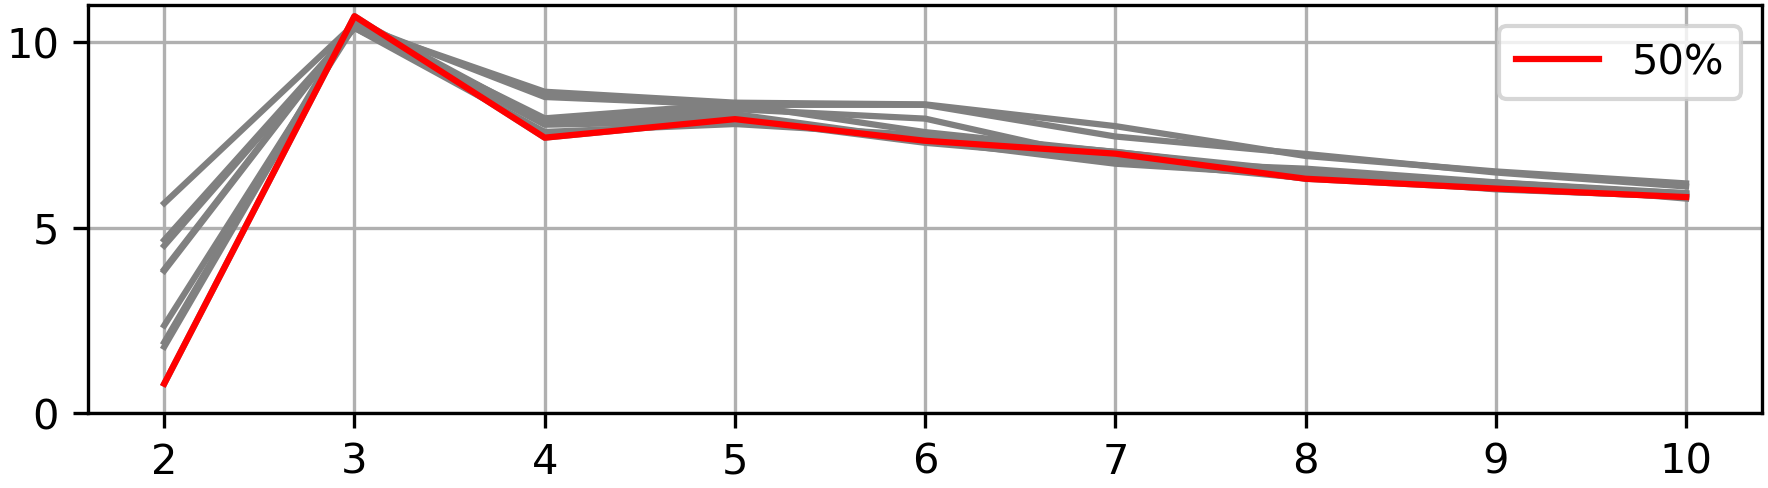
\includegraphics[width=0.8\linewidth]{pictures/Кластеры-дистанция}
	\\
	\caption{Дистанция, соотнесенная с числом кластеров}
\end{figure}
Усредним кривые дистанций. Для этого проведем усреднение по столбцам сводной таблицы:

\noindent
%---------------------------------------
%---------------------------------------
\SetTblrInner{rowsep=3pt}
%---------------------------------------
\begin{longtblr}
	{
		colspec = {
			X[r,f]
			X[r,f] 
			X[r,f] 
			X[r,f] 
			X[r,f]
			X[r,f]
			X[r,f] 
			X[r,f] 
			X[r,f] 
			X[c,f]
		},
		width = \linewidth,
		rowhead = 1, 
		rowfoot = 0,
		row{odd} = {}, 
		row{even} = {},
		rows    = {font=\scriptsize},
		row{1}  = {font=\scriptsize\bfseries}
	}
	&
	10\%
	& 
	20\%
	&
	30\%
	&
	40\%
	& 
	50\%
	&
	60\%
	& 
	70\%
	&
	80\%
	&
	90\%
	\\
	\hline[1pt]
	\textbf{}   
	&7.3948	&7.1699	&7.1487	&6.7341	&6.5953	&6.7863	&7.0113	&7.0893	&7.2802
	\\
	\hline[1pt]
\end{longtblr}
%---------------------------------------
\noindent
После усреднения кривые становятся горизонтальными линиями. Низшая линия соответствует проценту тестовой выборки с наилучшим значением нашей метрики (см. рис.~2).
\begin{figure}[!h]
	\centering
	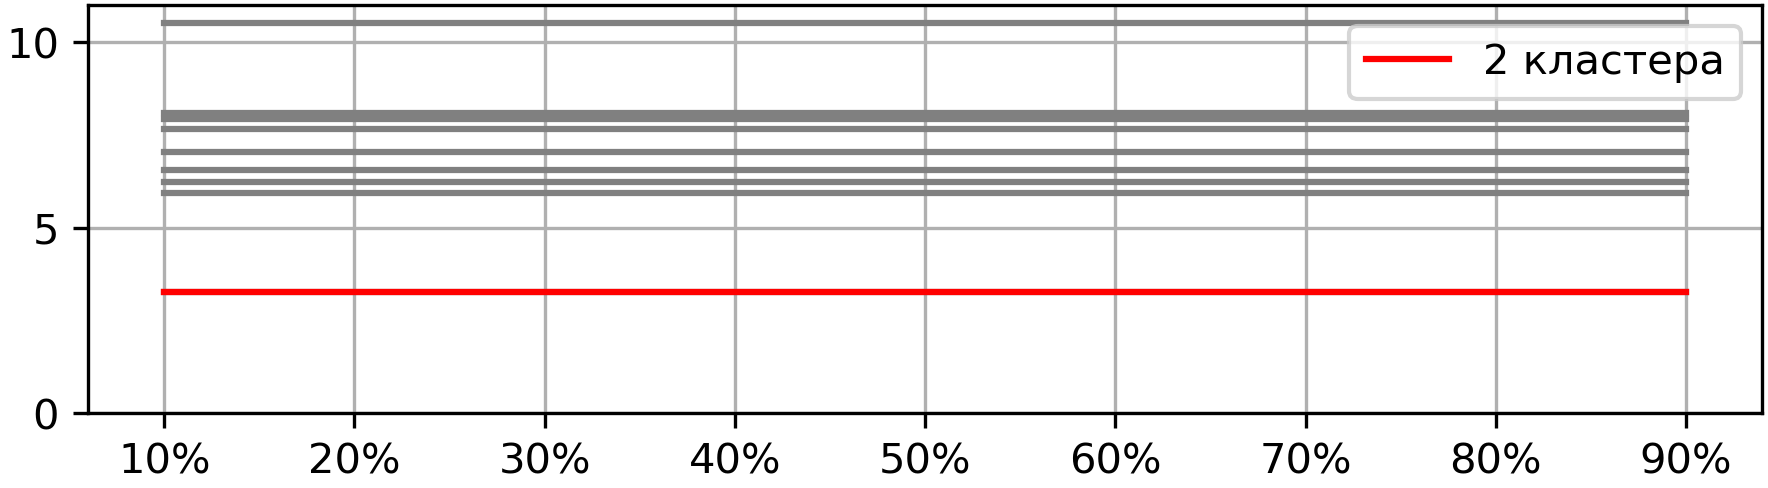
\includegraphics[width=0.8\linewidth]{pictures/Проценты-дистанция. Средние}
	\\
	\caption{ Дистанция, усредненная по всем процентам test'а}
\end{figure}
Таким образом, наименьшее отклонение центроидов происходит при разбиении выборки в пропорции 50\%:50\%.

\subsection{Анализ по объему тестовой выборки}

Аналогично мы можем визуализировать дистанции между центроидами, соотнеся их с процентом тестовой выборки (см. рис. 3). Здесь девять кривых соответствуют девяти строкам сводной таблицы, и каждая кривая описывает ситуацию при фиксированном числе кластеров, на которые производится разбиение данных (от 2 до 10).
\begin{figure}[!h]
	\centering
	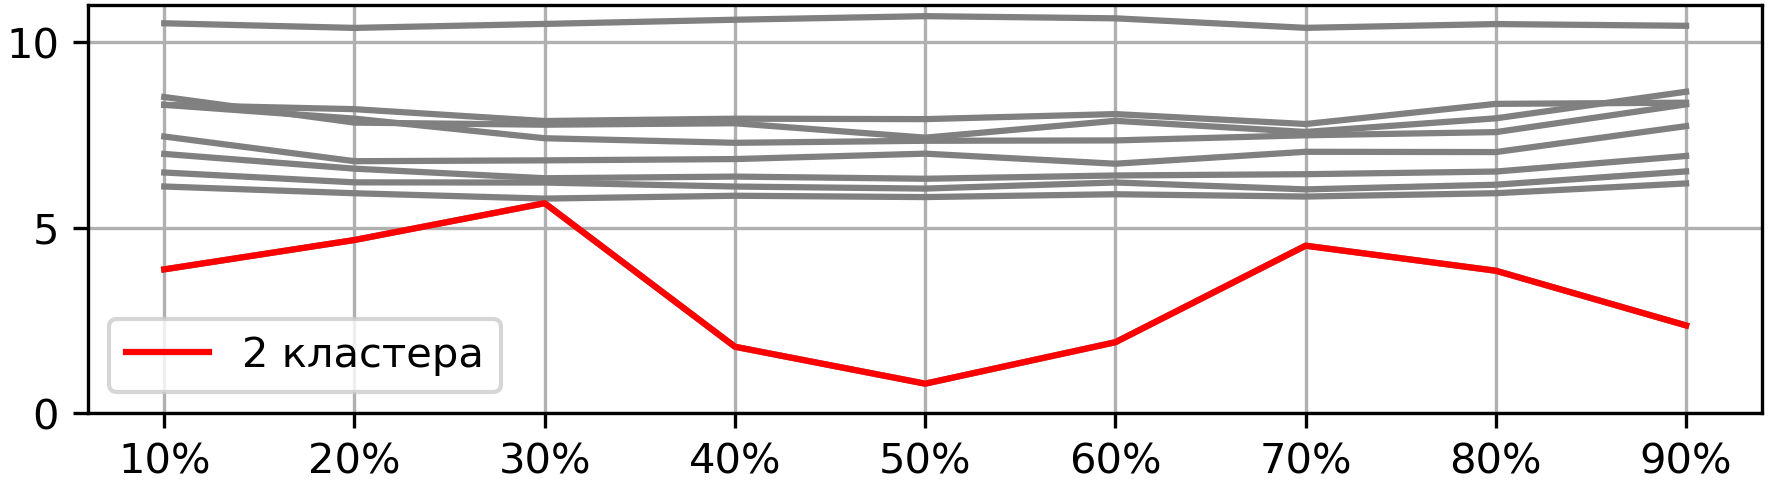
\includegraphics[width=0.8\linewidth]{pictures/Проценты-дистанция}
	\\
	\caption{Дистанция, соотнесенная с процентом тестовой выборки}
\end{figure}

Так же как и выше усредняем кривые дистанций. Для этого вычисляем средние значения по строкам сводной таблицы:
\noindent
%---------------------------------------
%---------------------------------------
\SetTblrInner{rowsep=3pt}
%---------------------------------------
\begin{longtblr}
	{
		colspec = {
			X[r,f]
			X[r,f] 
			X[r,f] 
			X[r,f] 
			X[r,f]
			X[r,f]
			X[r,f] 
			X[r,f] 
			X[r,f] 
			X[c,f]
		},
		width = \linewidth,
		rowhead = 1, 
		rowfoot = 0,
		row{odd} = {}, 
		row{even} = {},
		rows    = {font=\scriptsize},
		row{1}  = {font=\scriptsize\bfseries}
	}
	&
	2
	& 
	3
	&
	4
	&
	5
	& 
	6
	&
	7
	& 
	8
	&
	9
	&
	10
	\\
	\hline[1pt]
	\textbf{}   
	&3.2628	&10.5178	&7.9365	&8.0881	&7.6685	&7.0478	&6.5416	&6.2203	&5.9264
	\\
	\hline[1pt]
\end{longtblr}
%---------------------------------------
\noindent
В результате получаем серию горизонтальных линий. Низшая линия соответствует числу кластеров с наилучшим значением нашей метрики.
\begin{figure}[!h]
	\centering
	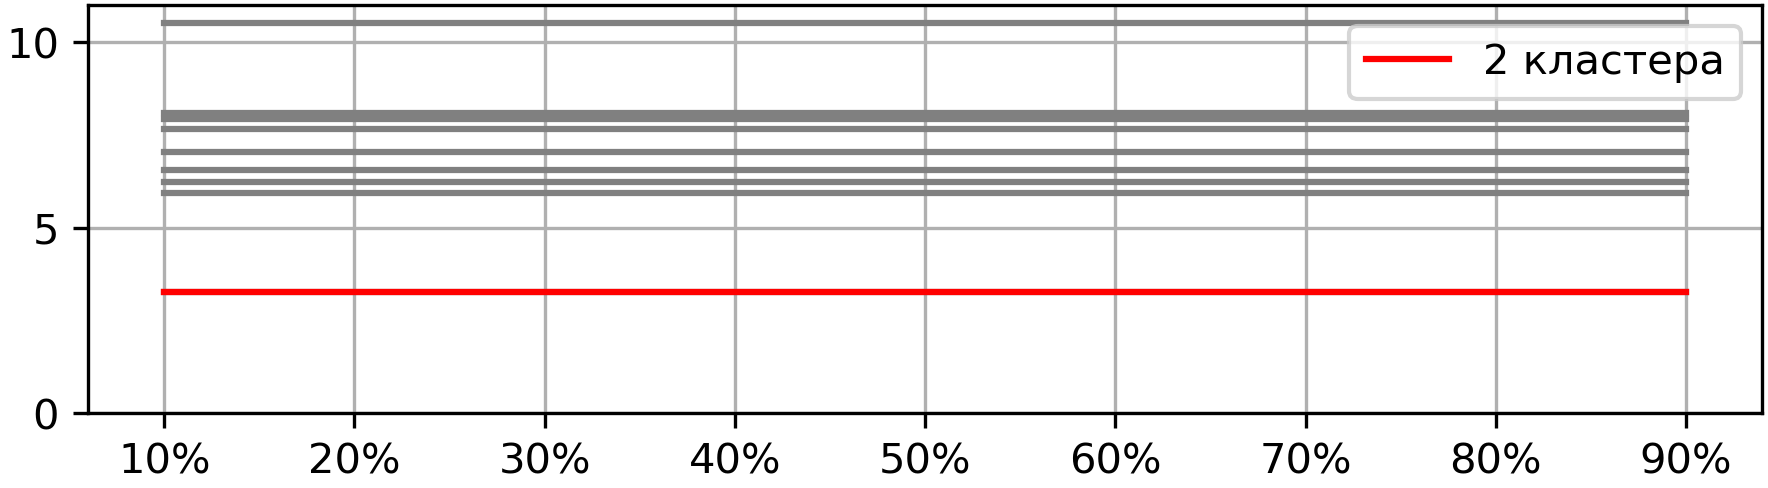
\includegraphics[width=0.8\linewidth]{pictures/Проценты-дистанция. Средние}
	\\
	\caption{Дистанция, усредненная по всем кластерам}
\end{figure}

\noindent
Таким образом, оптимальное число кластеров равно 2.

\section{Выводы}

В большинстве задач машинного обучения нет заранее известной информации о количестве кластеров в данных, поэтому их число должно быть определено на основе самих данных. Это делает процесс определения оптимального количества кластеров весьма сложным и неоднозначным. Существует множество методов и метрик для определения оптимального числа кластеров (см. [2]), но в данной работе мы предложили и апробировали собственный метод, основанный на средних дистанциях между центроидами кластеров на обучающей и тестовой выборке. Предложенный нами метод подбора оптимального числа кластеров для агломеративной кластеризации показал хорошую работоспособность, четко выделив сразу два показателя: 1) оптимальное количество кластеров, 2) оптимальную пропорцию для разбиения данных на обучающую и тестовую выборку. 

\section{Литература}

\begin{enumerate}
	\item Хейдт М. Изучаем Pandas / М. Хейдт;  — Москва: ДМК Пресс, 2018. — 438 с.
	\item Бурков А. Машинное обучение без лишних слов / А. Бурков;  — СПб: Питер, 2020. — 192 с.
	\item .Вьюгин, В. В. Математические основы теории машинного обучения и прогнозирования / В. В. Вьюгин; — М.: МЦИМО. — 2013. — 387~с.
	\item Бринк Х. Машинное обучение / Х. Бринк, Дж. Ричардс, М. Феверолф  — СПб.: Питер, 2017. — 336 с.
	\item Байков И.И., Семерова Е.А., Курмуков А.И. Метод ансамблирования алгоритмов кластеризации для решения задачи совместной кластеризации // Сенсорные системы. 2021. Т. 35. № 1. С. 43--49.
	\item Паксашвили С.А. тестирования алгоритма кластеризации k-means в решении задачи кластеризации финансовых операций // В сборнике: СНК-2022. Материалы LXXII открытой международной студенческой научной конференции Московского Политеха. Москва, 2022. С. 347--353.
\end{enumerate}



\end{document}
